\documentclass[a4paper,12pt,twocolumn]{article}
\usepackage[utf8]{inputenc}
\usepackage{amsmath}
\usepackage{graphicx}
\usepackage{hyperref}
\usepackage[margin=0.5in]{geometry}
\title{Assignment-1- Canonical PoS using Platformio}
\author{Ravi Sumanth Muppana- FWC22003}
\date{August 2022}

\begin{document}

\maketitle

\section{Problem:}
Derive a Canonical POS expression for a Boolean function F, represented by the following truth table:

\begin{figure}[h]
\centering
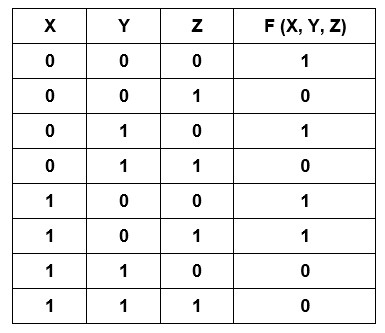
\includegraphics[width=1.0\columnwidth]{TT-document}
\label{Truth Table}
\end{figure}
\maketitle\section{Solution:}
\subsection{Theory:}
Canonical form is simply representing the Boolean function as sum of minimum terms (SoP) or product of maximum terms (PoS). For canonical PoS form, consider the input rows where the output is '0' and do logical AND of all those max terms in order to get the Boolean expression function.\\
There are four cases where the output is '0'. They are [(0,0,1),(0,1,1),(1,1,0),(1,1,1)]. 
\subsection{Boolean expression:}
$F(X,Y,Z)=(X+Y+Z').(X+Y'+Z').$\\$(X'+Y'+Z).(X'+Y'+Z')$

\newpage
\subsection{Components:} 
\begin{figure}[h]
\centering
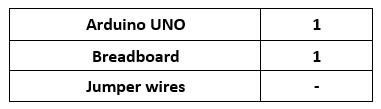
\includegraphics[width=1\columnwidth]{TT-2-document}
\label{Truth Table}
\end{figure}
\subsection{Connections:}
Arduino UNO has LED connected to Pin 13. Let pins 6,7,8 be the inputs. Connect the input pin to Vcc, if it must be set to '1'. Connect the input pin to GND of arduino board, if it must be set to '0'. The LED will glow if the output is '1'. 
\section{Software:}
Download this pdf and click on the below link for source code:\\
\href{https://raw.githubusercontent.com/Ravisumanth/FWC-1/main/assignment.cpp}{Source file link}






\end{document}
